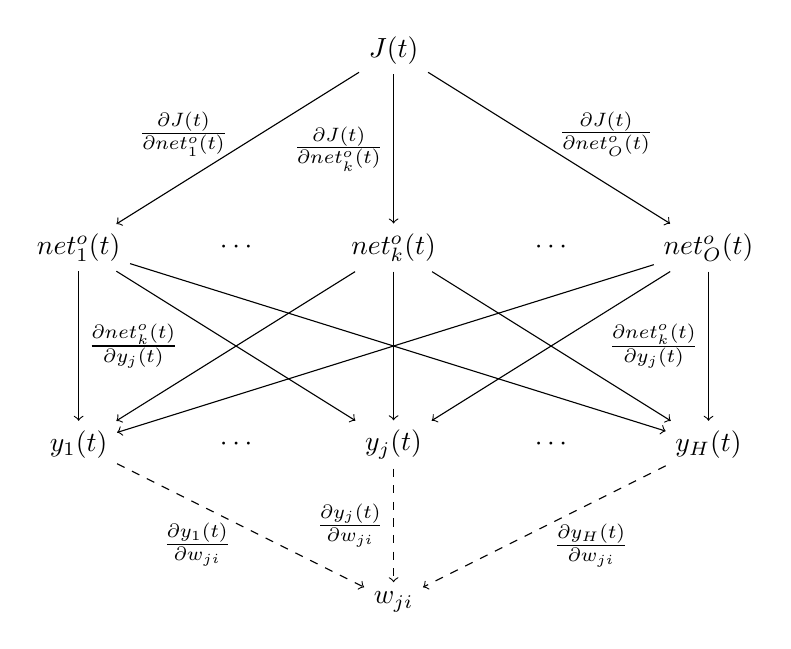
\begin{tikzpicture}
    \node (J) at ( 0,  0) {$J(t)$}; 
    
    \node (netk1) at ( -4, -2.5) {$net^o_1(t)$};
    \node (netk1k) at ( -2, -2.5) {$\cdots$};
    \node (netk) at ( 0, -2.5) {$net^o_k(t)$};
    \node (netkkn) at ( 2, -2.5) {$\cdots$};
    \node (netkn) at ( 4, -2.5) {$net^o_O(t)$};
   
    \node (y1) at ( -4, -5) {$y_1(t)$}; 
    \node (y1j) at ( -2, -5) {$\cdots$};
    \node (yj) at ( 0, -5) {$y_j(t)$};
    \node (yjH) at ( 2, -5) {$\cdots$};
    \node (yH) at ( 4, -5) {$y_H(t)$};
    
     \node (wji) at ( 0, -7) {$w_{ji}$};
    
    \begin{scope}[every path/.style={->}]
       \draw (J) -- node [above=.5em, left] {$\frac{\partial J(t)}{\partial net^o_1(t)}$} (netk1);
       \draw (J) -- node [left] {$\frac{\partial J(t)}{\partial net^o_k(t)}$} (netk);
       \draw (J) -- node [above=.5em, right] {$\frac{\partial J(t)}{\partial net^o_O(t)}$} (netkn);
       
       \draw (netk1) -- node [right] {$\frac{\partial net^o_k(t)}{\partial y_j(t)}$} (y1);
       \draw (netk) --  (y1);
       \draw (netkn) -- (y1);
       
       \draw (netk1) -- (yj);
       \draw (netk) -- (yj);
       \draw (netkn) -- (yj);
       
       \draw (netk1) --  (yH);
       \draw (netk) -- (yH);
       \draw (netkn) -- node [left] {$\frac{\partial net^o_k(t)}{\partial y_j(t)}$} (yH);
       
       \draw[dashed] (y1) -- node [solid, below=.7em,  left] {$\frac{\partial y_1(t)}{\partial w_{ji}}$}  (wji);
       \draw[dashed] (yj) -- node [solid, left] {$\frac{\partial y_j(t)}{\partial w_{ji}}$}  (wji);
       \draw[dashed] (yH) -- node [solid, below=.7em, right] {$\frac{\partial y_H(t)}{\partial w_{ji}}$}  (wji);
    \end{scope} 
\end{tikzpicture}

